\documentclass[12pt]{article}
\usepackage{tikz}
\usetikzlibrary{angles,quotes}

% global styles
\tikzset{help lines/.style={color=gray!50,very thin,step=.5}}

\begin{document}
First tikz picture.

\begin{center}
  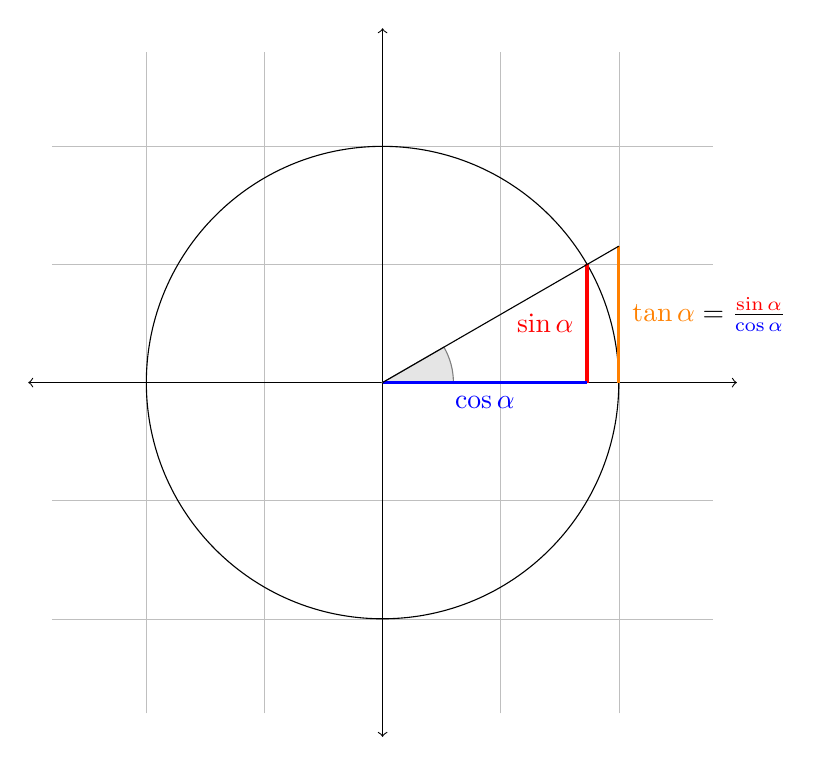
\begin{tikzpicture}[scale=3]
    % axis y grid
    \draw[help lines] (-1.4,-1.4) grid (1.4,1.4);
    \draw[<->] (-1.5,0) -- (1.5,0);
    \draw[<->] (0,-1.5) -- (0,1.5);

    % circle
    \draw (0,0) circle [radius=1cm];

    % angle shadow
    \filldraw[fill=gray!20,draw=black!50] (0,0) -- (3mm,0) arc [start angle=0, end angle=30, radius=3mm] -- cycle;

    % sine
    \draw[red, very thick] (30:1cm) -- node[left=1pt] {$\sin \alpha$} +(0,-0.5);

    % cosine
    \draw[blue, very thick] (30:1cm) +(0,-0.5) -- node[below=1pt] {$\cos \alpha$} (0,0);

    % tangent
    \draw[orange, very thick] (1,0) -- node[right=1pt] {$\tan \alpha \color{black}= \frac{\color{red}\sin \alpha}{\color{blue}\cos \alpha}$} (1,{tan(30)});

    % hypotenuse
    \draw (0,0) -- (1,{tan(30)});
  \end{tikzpicture}
\end{center}

Pic templating.

\begin{center}
  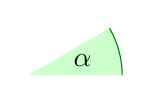
\begin{tikzpicture}[scale=3]
    \coordinate (A) at (1,0);
    \coordinate (B) at (0,0);
    \coordinate (C) at (30:1cm);

    \draw pic [draw=green!50!black, fill=green!20, angle radius=12mm,
    "$\alpha$"] {angle = A--B--C};
  \end{tikzpicture}
\end{center}
\end{document}
